\begin{figure}
    \centering
    \caption{Logarithmic Energy consumption of the Raspberry Pi.}
    \label{fig:log-rpi-energy}
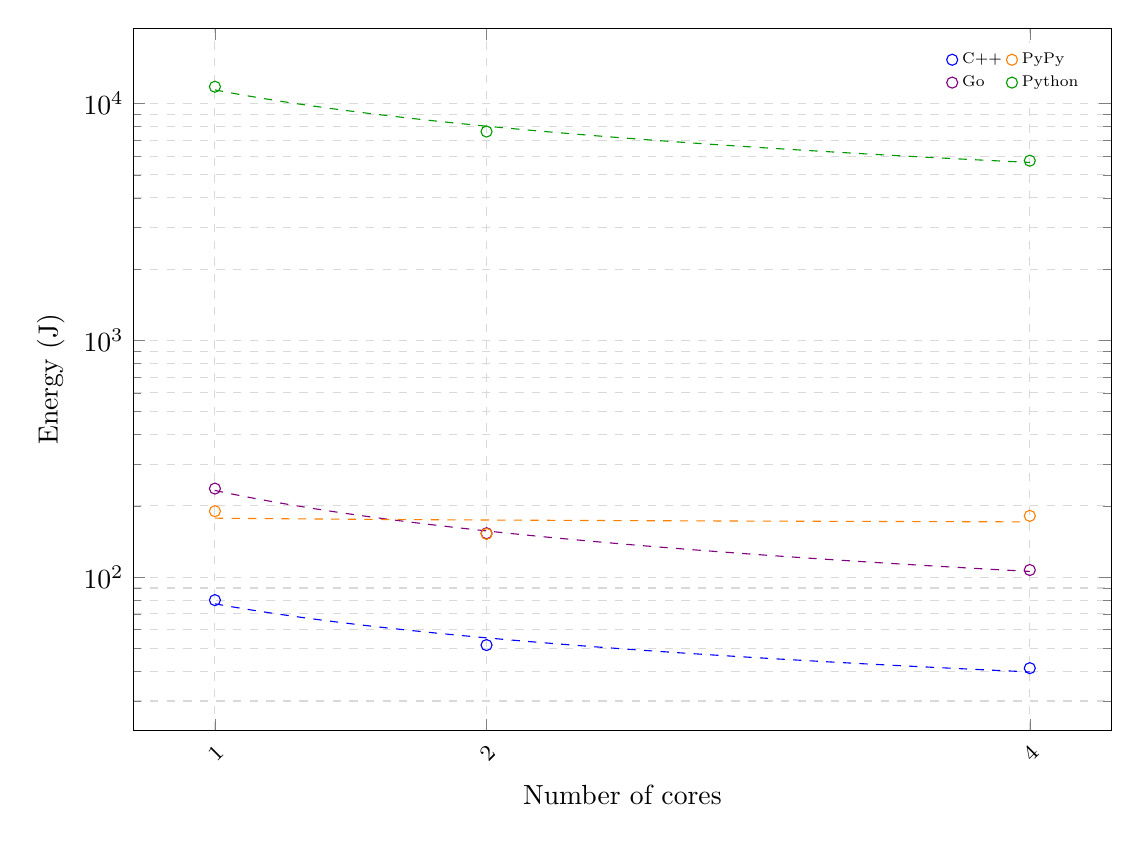
\begin{tikzpicture}
  \begin{semilogyaxis}[
      width=14cm,
      height=10.5cm,
      xlabel={Number of cores},
      ylabel={Energy (J)},
      ymode=log,
      xmode=linear,
      grid=both,
      minor tick num=1,
      grid style={gray!30,dashed},
      xtick={1,2,4},
      x tick label style={
        font=\footnotesize,
        rotate=45,
        anchor=north east
      },
      legend style={
        at={(0.98,0.98)},
        anchor=north east,
        font=\scriptsize,
        nodes={scale=0.8,transform shape},
        draw=none
      },
      legend columns=2,
      transpose legend,
      legend cell align=left,
    ]

    %% C++ %%
    \addplot[
      blue, only marks, mark=o,
      mark options={draw=blue,fill=white}
    ]
    table[row sep=\\] {
      x   y     \\
      1   80.00  \\
      2   51.67  \\
      4   41.28  \\
    };
    \addlegendentry{C++}
    % fit: y = 77.2 * x^{-0.478}
    \addplot[
      blue, dashed, forget plot,
      domain=1:4, samples=200
    ] {77.2 * x^(-0.478)};

    %% Go %%
    \addplot[
      violet, only marks, mark=o,
      mark options={draw=violet,fill=white}
    ]
    table[row sep=\\] {
      x    y       \\
      1    236.67  \\
      2    153.33  \\
      4    107.20  \\
    };
    \addlegendentry{Go}
    % fit: y = 232.4 * x^{-0.568}
    \addplot[
      violet, dashed, forget plot,
      domain=1:4, samples=200
    ] {232.4 * x^(-0.568)};

    %% PyPy %%
    \addplot[
      orange, only marks, mark=o,
      mark options={draw=orange,fill=white}
    ]
    table[row sep=\\] {
      x    y      \\
      1    190.00 \\
      2    152.33 \\
      4    181.60 \\
    };
    \addlegendentry{PyPy}
    % fit: y = 177.5 * x^{-0.026}
    \addplot[
      orange, dashed, forget plot,
      domain=1:4, samples=200
    ] {177.5 * x^(-0.026)};

    %% Python %%
    \addplot[
      green!60!black, only marks, mark=o,
      mark options={draw=green!60!black,fill=white}
    ]
    table[row sep=\\] {
      x      y        \\
      1      11780.00 \\
      2      7620.67  \\
      4      5739.00  \\
    };
    \addlegendentry{Python}
    % fit: y = 11423 * x^{-0.509}
    \addplot[
      green!60!black, dashed, forget plot,
      domain=1:4, samples=200
    ] {11423 * x^(-0.509)};

  \end{semilogyaxis}
\end{tikzpicture}
\end{figure}

\begin{table}
    \centering
    \begin{tabular}{lrrrr}
        \hline
        Cores & C++    & Go      & PyPy         & Python      \\
        \hline
        1     & 80.00  & 236.67  & 190.00       & 11\,780.00  \\
        2     & 51.67  & 153.33  & 152.33       &  7\,620.67  \\
        4     & 41.28  & 107.20  & 181.60       &  5\,739.00  \\
        \hline
    \end{tabular}
    \caption{Power‐sum (J) by implementation and core count}
    \label{tab:power-sum-by-cores}
\end{table}